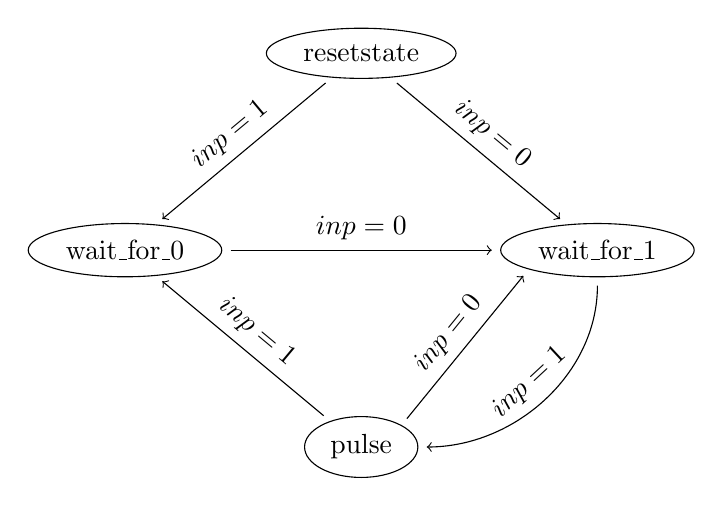
\begin{tikzpicture}
	\usetikzlibrary{shapes}
	\tikzset{state/.style={draw, ellipse, align=center}}
	\tikzset{arrow/.style={draw, ->, shorten >=3pt, shorten <=3pt}}
	
	\node[state] (a) at (0, 2.5) {resetstate};
	\node[state] (b) at (3, 0) {wait\_for\_1};
	\node[state] (c) at (0, -2.5) {pulse};
	\node[state] (d) at (-3, 0) {wait\_for\_0};
	

	\draw[arrow] (a) -- node[sloped, anchor=center, above] {$inp=0$} (b);
	\draw[arrow] (a) -- node[sloped, anchor=center, above] {$inp=1$} (d);
	
	\draw[arrow, out=-90, in=0] (b.south) to node[sloped, anchor=center, above] {$inp=1$} (c.east);
	
	\draw[arrow] (c.north east) -- node[sloped, anchor=center, above] {$inp=0$} (b.south west);
	
	\draw[arrow] (c) -- node[sloped, anchor=center, above] {$inp=1$} (d);
	\draw[arrow] (d) -- node[sloped, anchor=center, above] {$inp=0$} (b);
\end{tikzpicture}
